%!TEX root = ../thesis.tex
% Spellcheck ignore
% cSpell:ignore midskip, Teledyne, Lecroy,oscilloscope, piezo, smallskip, dialimitplot, FWHM, diaminplot, meanplot, diaplot, Irange, wavemeter, rbcell, centi, extracolsep, toprule, midrule, bottomrule, milli, eqref, detuning, photodiode, Toptica, photonics, nano, giga, collimated, bigskip, captionof, minipage, pagebreak, wincam, includegraphics,wrapfigure, ifpdf, graphicspath
%*******************************************************************************
%****************************** Third Chapter **********************************
%*******************************************************************************

\chapter{Experiment}

\ifpdf{}
    \graphicspath{{Chapter3/Figs/Raster/}{Chapter3/Figs/PDF/}{Chapter3/Figs/}}
\else
    \graphicspath{{Chapter3/Figs/Vector/}{Chapter3/Figs/}}
\fi

%********************************** % First Section  **************************************
\section{Laser} %Section - 3.1 

For all our measurements we used a \SI{420}{\nano\meter} DL (extended cavity laser
diode) pro HP laser with a 
DLC pro controller from Toptica photonics. An optical isolator (OI) is included
into the laser and thus the given powers are after OI\@.

\bigskip
\begin{table}[h]
    \centering
    \begin{tabular*}{0.6\textwidth}{@{\extracolsep{\fill} } l l}
    \toprule
    Specifications \\
    \midrule
    Wavelength: & \SI{421.0}{\nano\meter} \\
    Coarse Tuning: & \SI{419.5}{\nano\meter}~-~\SI{422.5}{\nano\meter} \\
    Max.~power: & \SI{78.0}{\milli\watt} \\
    At diode current: & \SI{93}{\milli\ampere} \\
    Mode Hop Free Tuning: & \SI{79}{\giga\hertz} at \SI{78.5}{\milli\ampere}\\
    \bottomrule
    \end{tabular*}
    \caption{\label{table:laser_spec} Specifications of Toptica DL pro HP 
    \SI{421}{\nano\meter}}
\end{table}

The laser has to be tuned to the right wavelength.
For that the beam was guided into a fiber and feeded into a wavemeter. The coarse 
tuning of the laser was done using the mechanical screw which changes the angle 
of the grating. Then the fine tuning was done playing both on the diode current
and the socket temperature on which the laser is mounted. To have a specific 
output power one would first adjust the diode current, which fines the power
and then readjust the temperature. \\
We characterized the beam profile \SI{50}{\centi\meter} after the beam outlet
(see Fig.~\ref{fig:beam50cm}), where we could see that the beam had a waist 
diameter of \(\approx\SI{933}{\micro\meter}\). It should be noted that the beam 
profile was not perfectly gaussian.

\begin{figure}
    \centering
    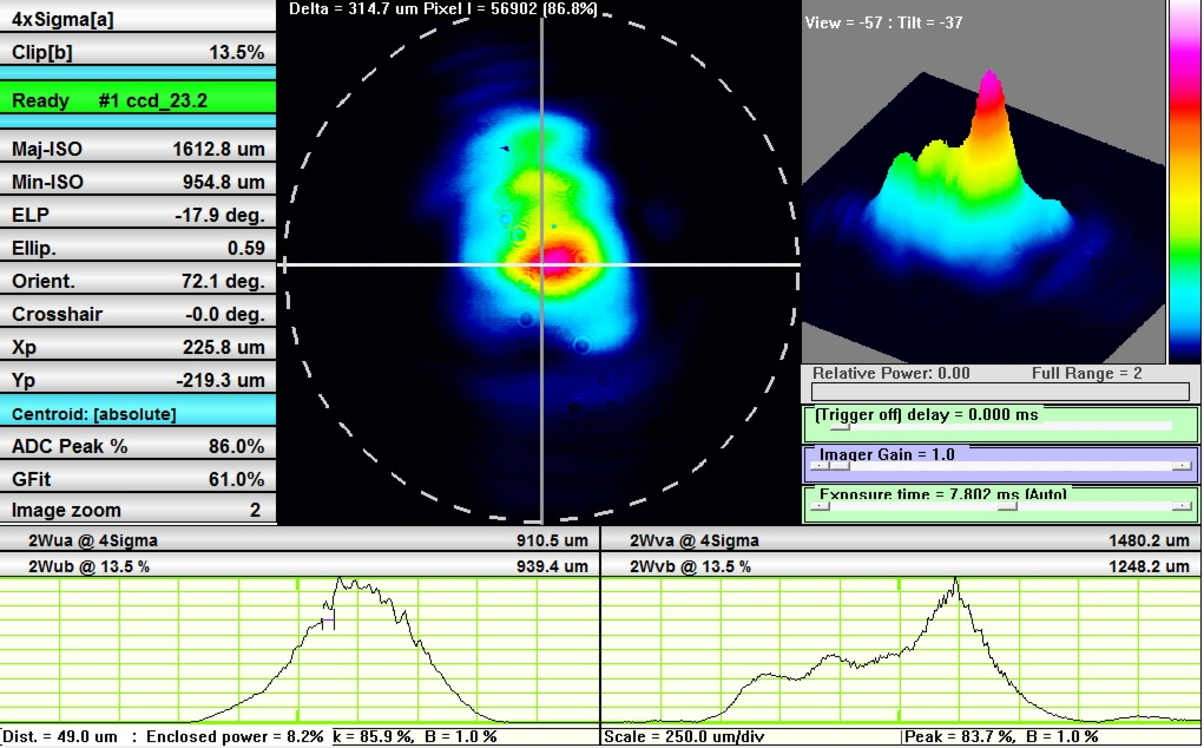
\includegraphics[width=.7\textwidth]{beam50cm}
    \caption{\label{fig:beam50cm} Beam profile after \SI{50}{\centi\meter}}
\end{figure}

%********************************** % Second Section  **************************************
\section{Setup} %Section - 3.2

\begin{figure}[H]
    \centering
    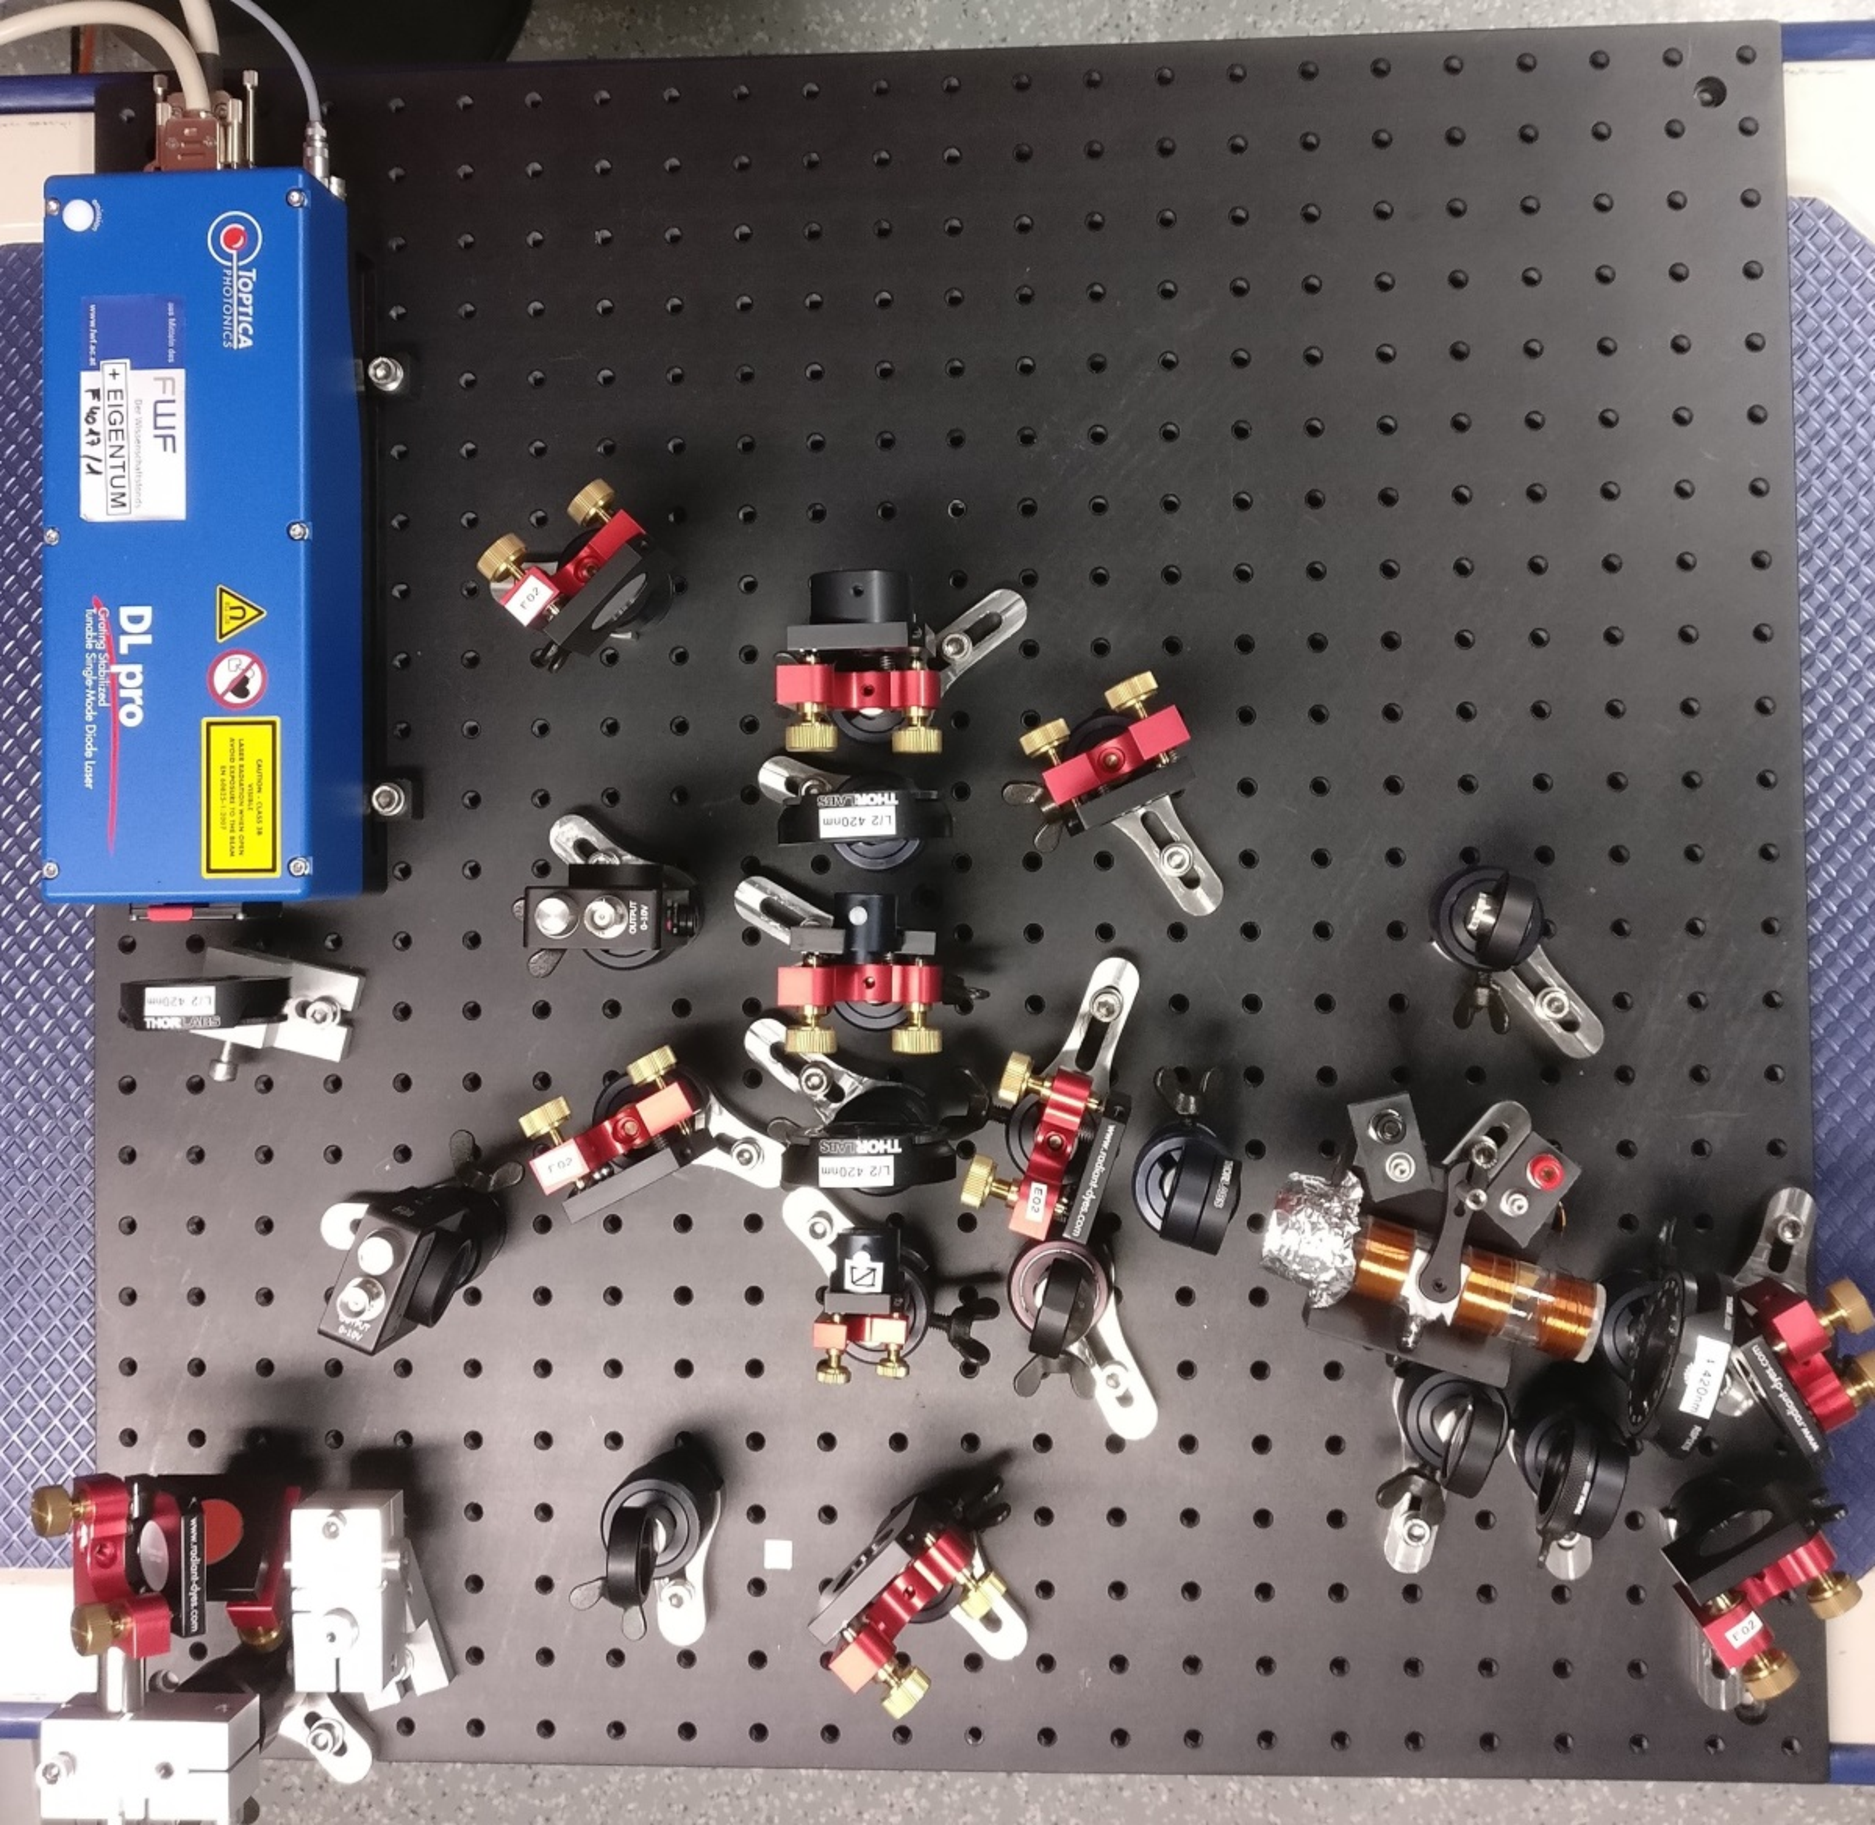
\includegraphics[width=.5\textwidth]{breadboard}
    \caption{\label{fig:breadboard} Setup mounted on a \(60 \times 60 \)\si{\centi\meter} 
    breadboard.}
\end{figure}

The laser bench should be placed on the experiment breadboard and thus, we took
into account space constraints when designing the beam path (see Fig.~\ref{fig:breadboard}).
The whole setup was mounted on a breadboard (\(60 \times 60 \)\si{\centi\meter}) 
and was divided into two parts via a polarization beam splitter (PBS) and a 
\(\lambda/2\) plate. Part of the beam power will be directed to the trap arm. 
This part was not built, we just placed a beam dump to block the beam, as can be 
seen in Fig.~\ref{fig:wincam_before}. But the occupied area had to be taken into 
account and we tried to built the spectroscopy setup (second arm) as compact as 
possible (see Fig.~\ref{fig:breadboard}).

\begin{figure}[H]
    \centering
    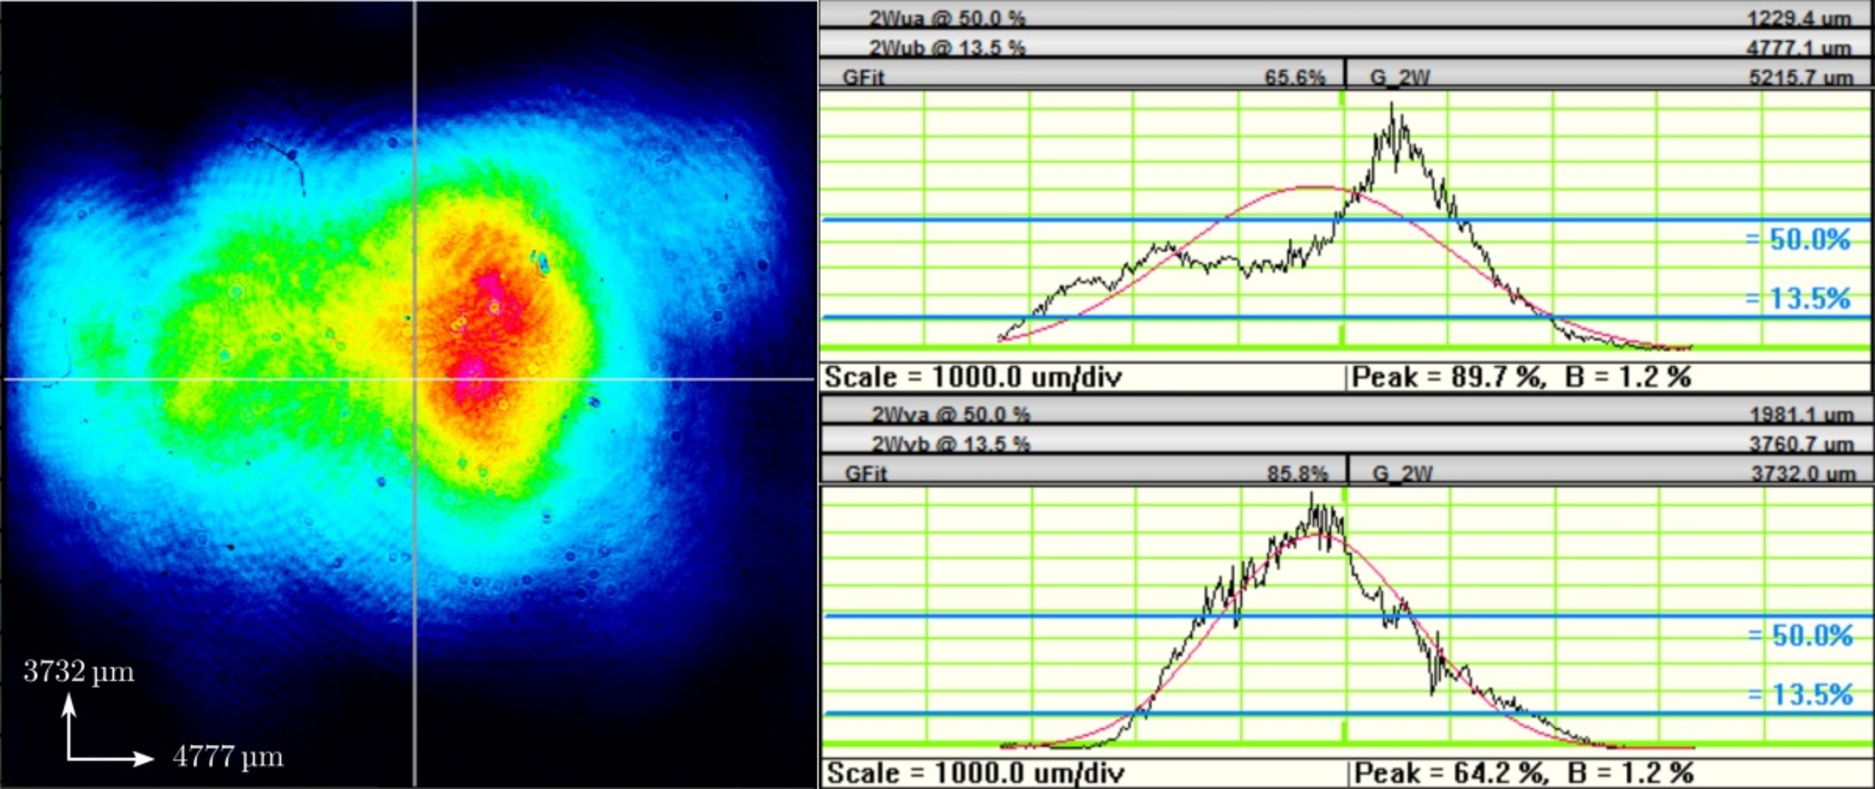
\includegraphics[width=0.7\textwidth]{beam_widened} 
    \caption{\label{fig:beam_widened} Beam profile after telescope setup.}
\end{figure}

We want to assume that all atoms receive the same intensity, such that we can 
use \(I = \frac{power}{cross~section} \). To achieve this, one has to change the 
beam profile by widening and additionally cropping to the center of the beam. 
To widen the beam we used a telescope setup after the PBS
with two lenses of different focal lengths (\(f_1 = \SI{2.5}{\centi\meter} 
\text{ and } f_2 = \SI{10}{\centi\meter}\)), which resulted in a beam with a waist
diameter of \(\approx \)\SI{3760}{\micro\meter} (see Fig.~\ref{fig:beam_widened}).
Therefore our magnification is \(\frac{3760}{933} = 4 = \frac{10}{2.5}\). Then 
the beam is cropped using an iris and guided through the cell with two mirrors. 
The iris aperture was chosen, in order to select the flat intensity.\\
The cell used in the setup is \SI{10}{\centi\meter} long and containing \(^{85}\)Rb
and \(^{87}\)Rb in isotopic concentrations. In order to increase absorption, we 
heated the rubidium cell with wire coils as seen in Fig.~\ref{fig:coils}. 
We used a wire with a diameter of \SI{0.315}{\milli\meter} for an higher resistance 
per unit of length. On the cell are four coils with \SI{35} turns each. The coils 
have alternating clock- and counter-clockwise windings, such that the generated 
magnetic fields cancel each other. The heater was operated with \SI{2}{\ampere} 
direct current to produce enough heat such that most of the condensed rubidium 
changed into the gas phase.

\begin{figure}[H]
    \centering
    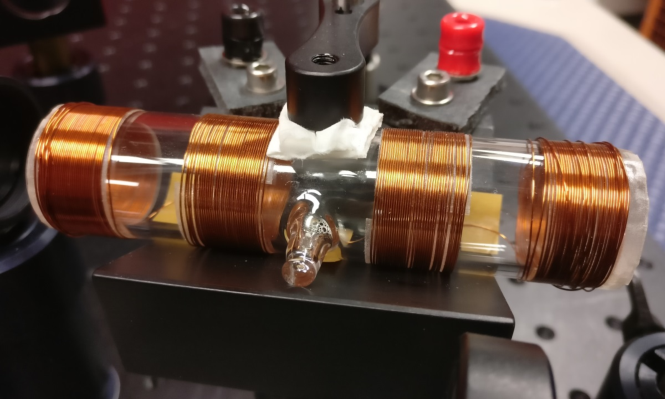
\includegraphics[width=.6\textwidth]{rbcell_coils}
    \caption{\label{fig:coils} Rubidium cell with applied copper wire coils for
    heating.}
\end{figure}


\pagebreak
%********************************** % Third Section  **************************************
\section{\label{sec:laser_dia_measurement}Laser diameter measurement} %Section - 3.3
\begin{minipage}[c]{.45\textwidth}
    \centering
    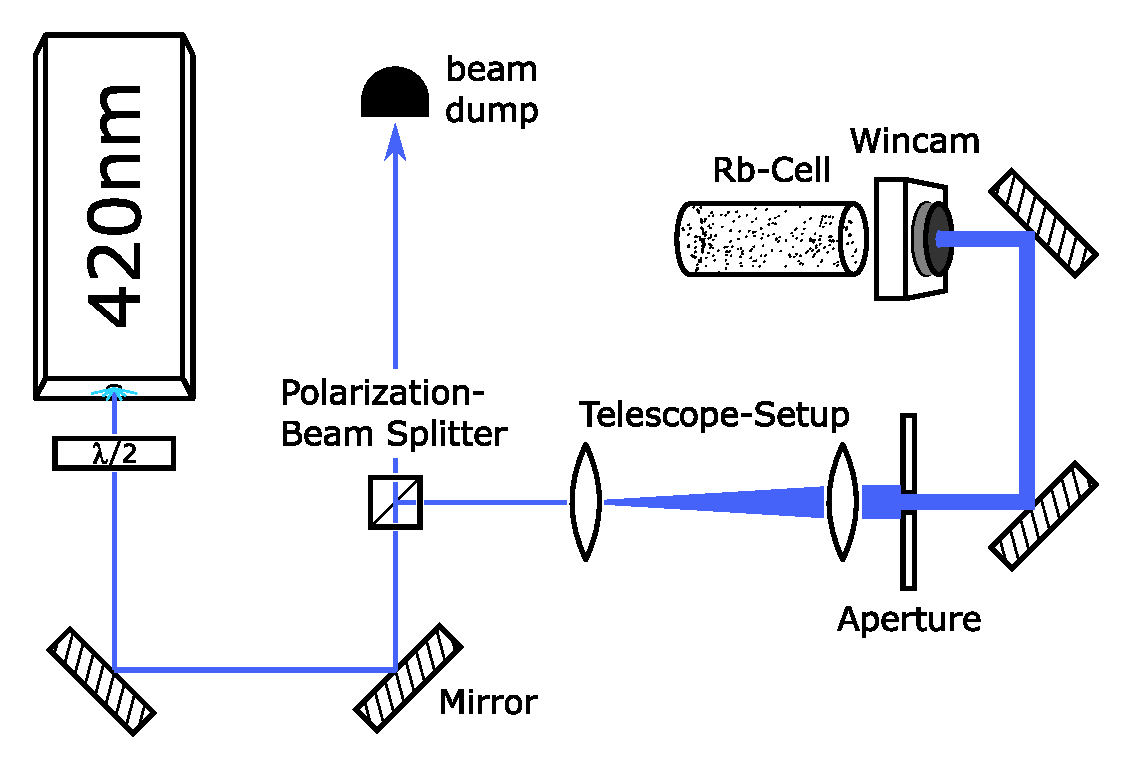
\includegraphics[width=.9\textwidth]{wincam_before}
    \captionof{figure}{\label{fig:wincam_before} Laser diameter measurement before 
    rubidium cell}
\end{minipage}
\hfill
\begin{minipage}[c]{.45\textwidth}
    \centering
    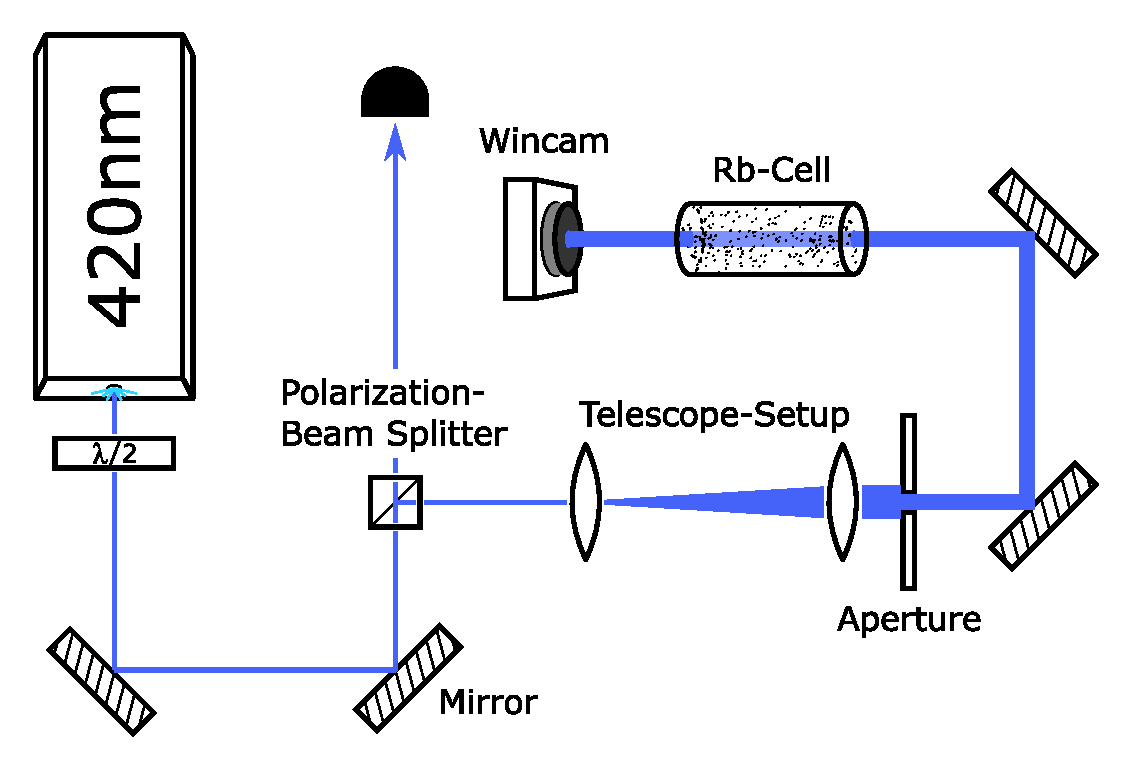
\includegraphics[width=.9\textwidth]{wincam_after}
    \captionof{figure}{\label{fig:wincam_after} Laser diameter measurement after 
    rubidium cell}
\end{minipage}

\begin{wrapfigure}{Hr}{.4\textwidth}
    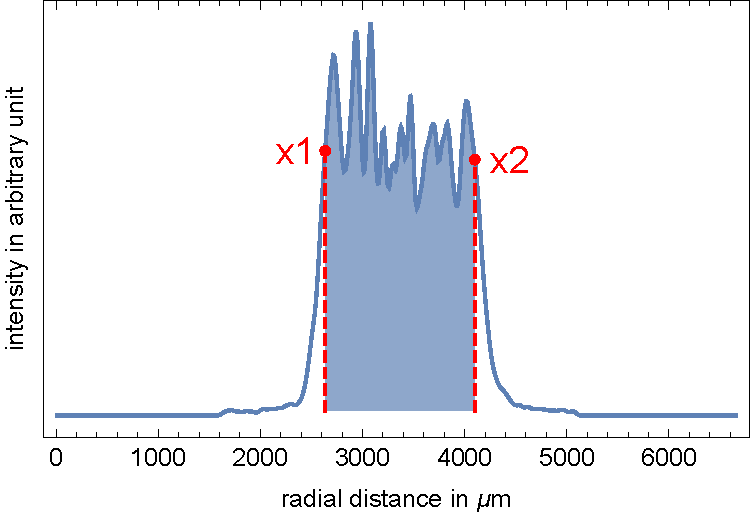
\includegraphics[width=0.33\textwidth]{dialimitplot}    
    \caption{\label{fig:diaminplot} By hand estimated beam limits.}
    \vspace{1em}
    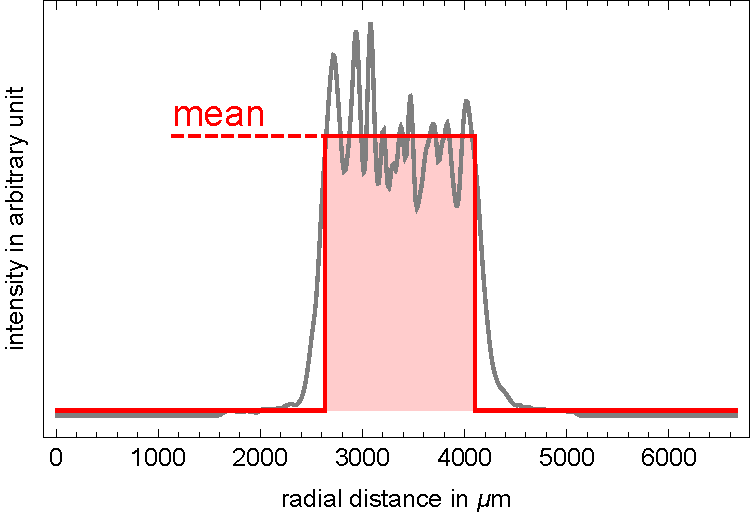
\includegraphics[width=0.33\textwidth]{meanplot}    
    \caption{\label{fig:meanplot} Equivalent flat hat beam.}
    \vspace{1em}
    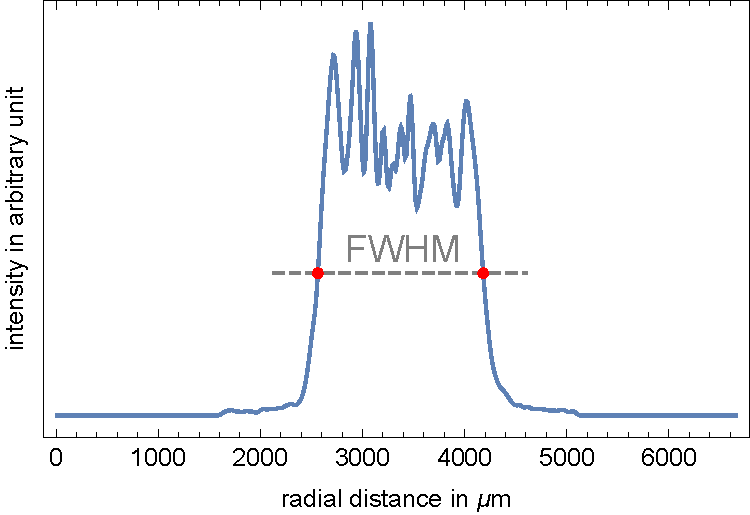
\includegraphics[width=0.33\textwidth]{diaplot}    
    \caption{\label{fig:diaplot} FWHM defines the estimated diameter.}
\end{wrapfigure}

\bigskip
In order to calculate the laser intensity one needs to measure the beam power and 
the beam cross section or rather the beam diameter. With a beam profiler (in our 
case a WinCamD) a measurement is performed in front and after the cell to measure 
and characterize the beam profile and check if the beam is collimated after the 
widening (see Fig.~\ref{fig:wincam_before}~and~\ref{fig:wincam_after}). 
The beam waist diameter calculated by the WinCamD application (see Fig.~\ref{fig:beam}) 
under the assumption of a gaussian beam is not correct. We will instead use a 
flat hat model for the evaluation and take the diameter where the power drops to 
half of the maximum power. It should be noted that the power is not constant over 
the whole beam profile, but shows \SI{30}{\percent} of fluctuations. We can then 
use the mean where the edge of the beam maximum is determined by hand. This leads 
to an uncertainty of \SI{+-100}{\micro\meter} per measurement. To obtain the 
equivalent flat hat intensity one has to integrate over the plot from limit to 
limit and divide by the interval (see Fig.~\ref{fig:meanplot}). The diameter of 
the beam is defined by its FWHM, this would be half the mean intensity as seen 
in Fig.~\ref{fig:diaplot}. The estimated beam diameter before the cell calculated 
out of the x- and y-axis slice is \SI[separate-uncertainty]{1608+-70}{\micro\meter} 
and \SI[separate-uncertainty]{1649+-70}{\micro\meter} after the cell. Therefore
the mean diameter is \SI[separate-uncertainty]{1628+-50}{\micro\meter} which
leads to an estimated cross section of
\SI[separate-uncertainty]{2.083+-0.128e-6}{\meter\squared}.


\pagebreak
\begin{figure}
    \centering
    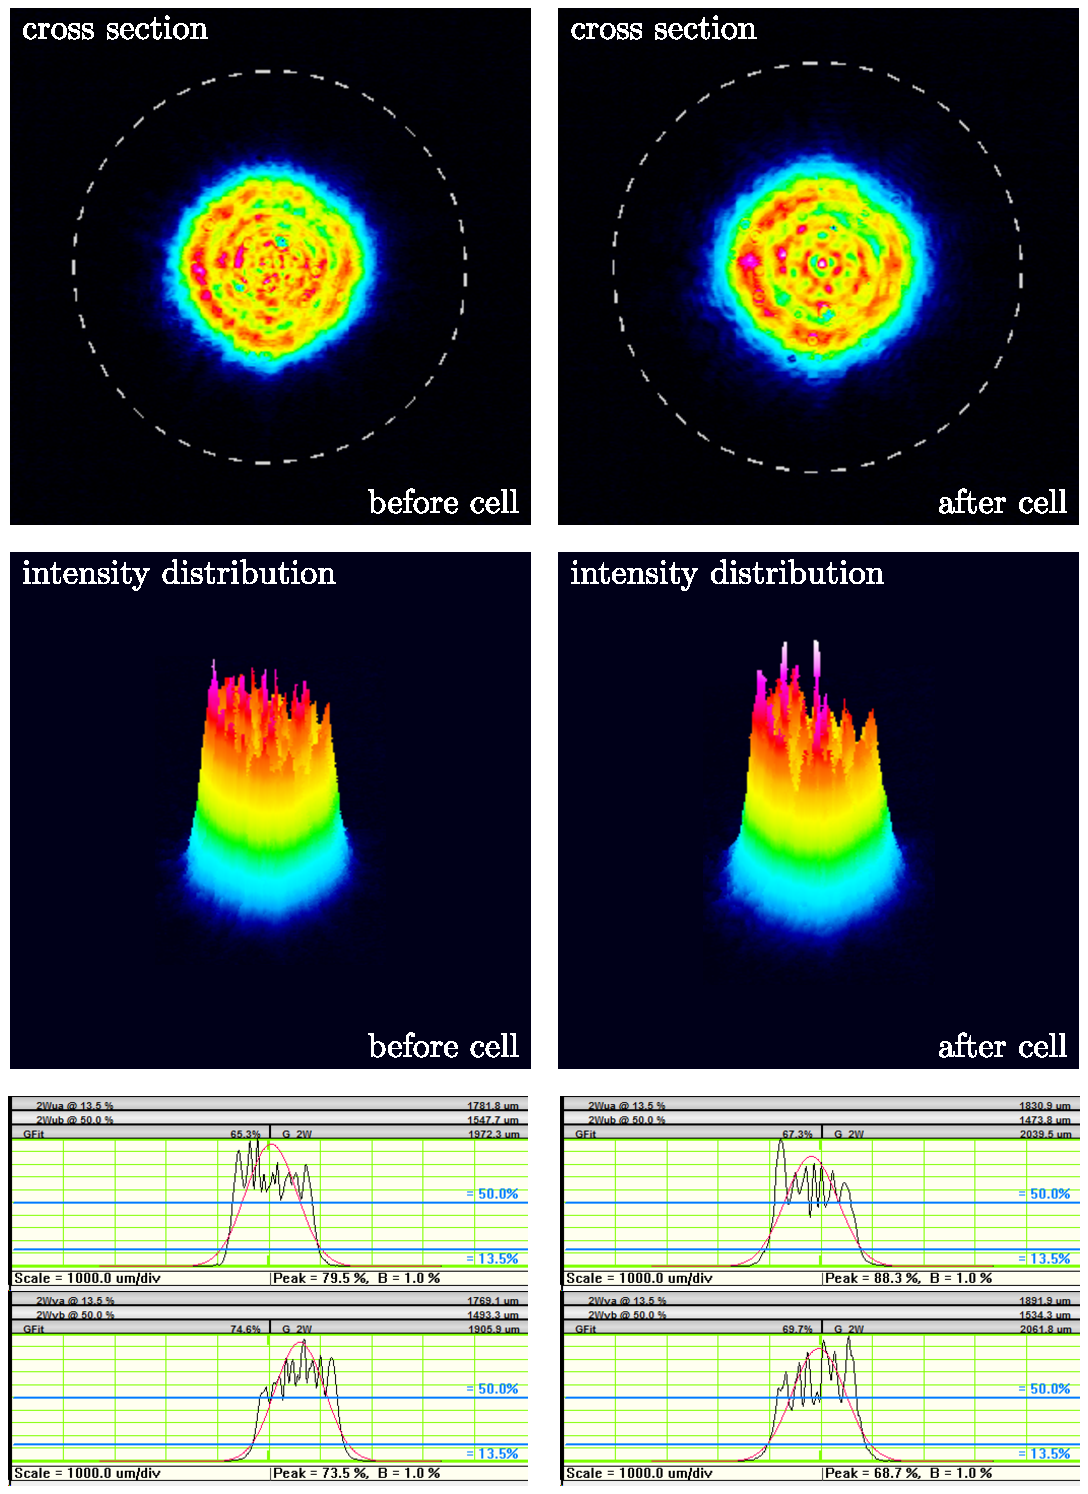
\includegraphics[width=.9\textwidth]{beam}
    \caption{\label{fig:beam} Cross section, intensity distribution and x- and 
    y-axes slices through beam center before and after cell transit.}
\end{figure}

\pagebreak
%********************************** % Forth Section  *************************************
\section{Absorption spectroscopy}\label{sec:absorption_spec} %Section - 3.4

\begin{figure}[!htb]
    \centering
    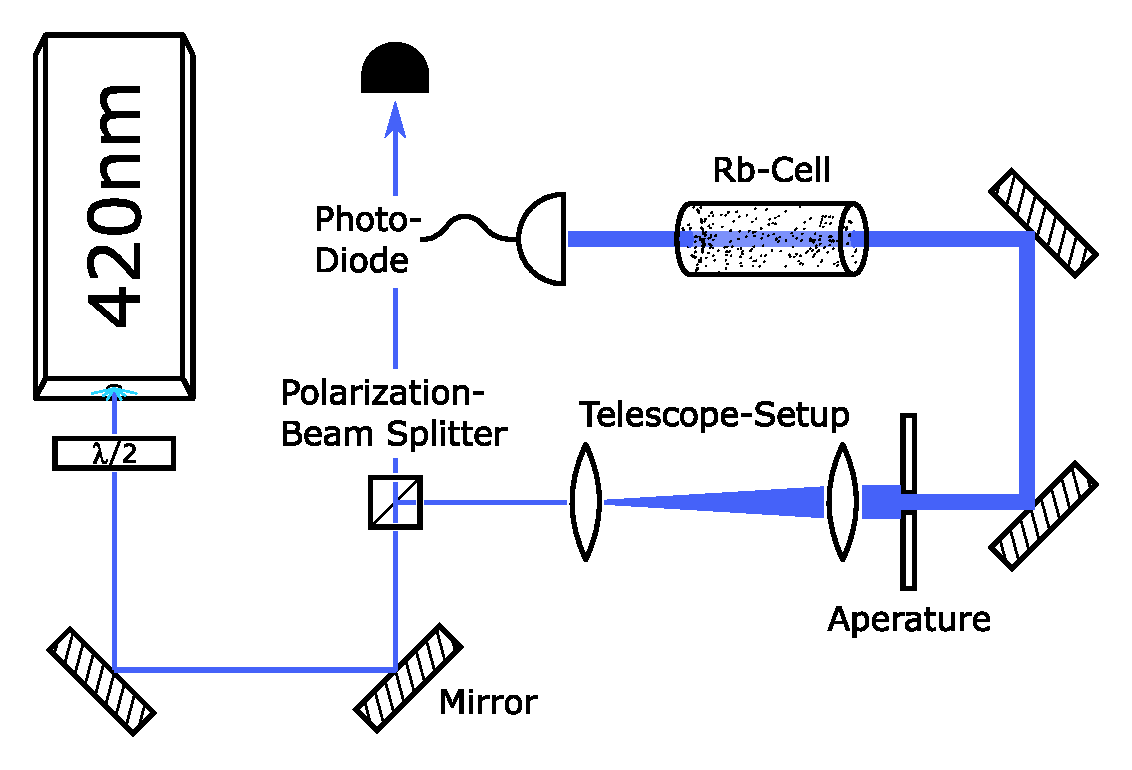
\includegraphics[width=0.6\textwidth]{absorption_spectroscopy}    
    \caption{\label{fig:absorption_spectroscopy_setup} Setup for an absorption 
    spectroscopy.}
\end{figure}

\begin{wrapfigure}{Hr}{.4\textwidth}
    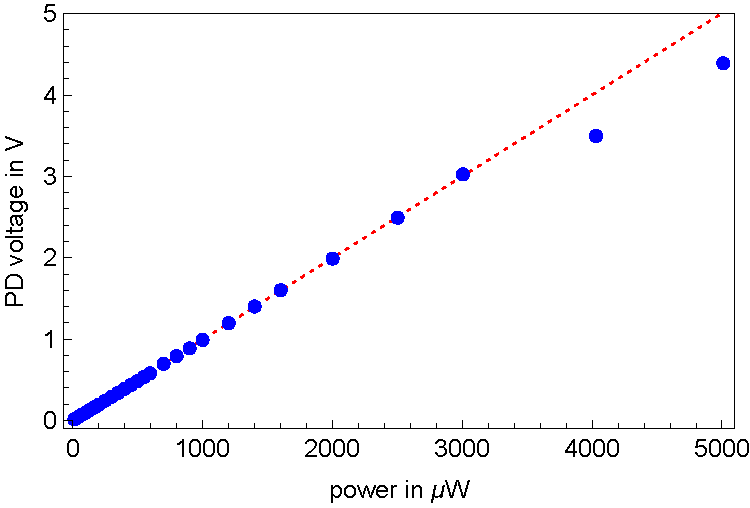
\includegraphics[width=0.35\textwidth]{pd_check}    
    \caption{\label{fig:pd_check} Maximum PD voltage taken out of atomic resonance 
    over power measured before the cell to ensure PD linearity; measurements at 
    \SI{4000}{\micro\watt} and \SI{5000}{\micro\watt} will be excluded.}
    \vspace{2em}
    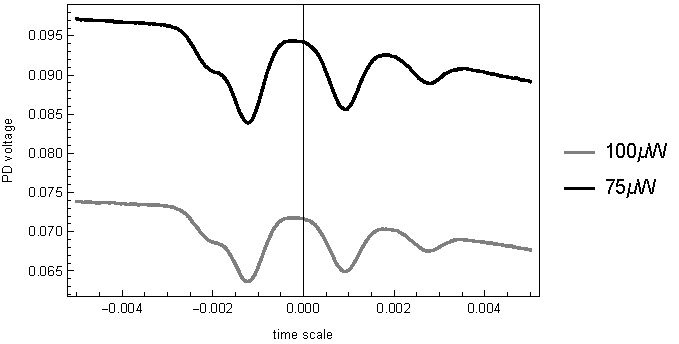
\includegraphics[width=0.35\textwidth]{power_compare}    
    \caption{\label{fig:power_compare} Absorption spectra at \SI{75}{\micro\watt}
    and \SI{100}{\micro\watt}.}
\end{wrapfigure}
We want to measure the intensity after the cell as a function of the initial
intensity \(I_0\). The transmitted intensity depends on the detuning as shown in
formula~\ref{eq:kappa_final}. \\
We will thus scan the laser frequency across the atomic resonances and for each 
input power record the signal using a photodiode (PD) 
(see Fig.~\ref{fig:absorption_spectroscopy_setup}) connected to a Teledyne Lecroy 
HDO6000A a digital storage oscilloscope. The PD records a signal 
proportional to the intensity only for a given range of power, so we made sure 
that we where using the PD in the linear range (see Fig.~\ref{fig:pd_check}). The
gain of the PD was adjusted in order to not saturate the signal, but to have the
widest possible dynamics to obtain the best signal to noise ratio. To 
change the input power, we turned the \(\lambda/2\) plate before the polarizing 
beam splitter (PBS) and measured it before every spectroscopy. It should be noted 
that changes of the sensor position in between measurements and variation of the
remaining ambient light lead to an increasing uncertainty at lower beam power. 
We account for \SI{10}{\percent} uncertainty below \SI{100}{\micro\watt}, 
\SI{8}{\percent} below \SI{250}{\micro\watt}, \SI{6}{\percent} below 
\SI{1000}{\micro\watt} and \SI{3}{\percent} above.\\
Before the spectroscopy itself, after the power was measured, the heating system,
due to its noise generating magnetic field, and all lights besides the measuring 
equipment were turned off. The spectroscopy was performed by scanning the laser 
wavelength using the piezo scanning option of the DL pro controller. We centered 
the scan range for all the measurements using the controller and the oscilloscope. 
For each input power we recorded the spectra and saved it onto a USB stick for 
further data analysis. We followed a logarithmic progression for the power 
increments from \SIrange{13}{5000}{\micro\watt}. Two examples of the recorded 
spectrum are shown in Fig.~\ref{fig:power_compare}. The choice of the power 
together with the beam cross section, should enable to probe intensity range from 
below to above \(I_{s}\). \\
In the next chapter we will discuss the analysis of the gathered data. 



